\section{Conversions d'énergie}\label{ex:conversion}

\begin{questions}
	\question Quelle conversion d'énergie est réalisée par une éolienne ? par un ventilateur électrique ?
		\begin{solution}
			Une éolienne convertit l'énergie cinétique en énergie électrique. Un ventilateur convertit l'énergie électrique en énergie cinétique.
		\end{solution}
	
	\question Réaliser la chaine énergétique correspondant à l'éolienne.
		\begin{solution}
			\begin{center}
				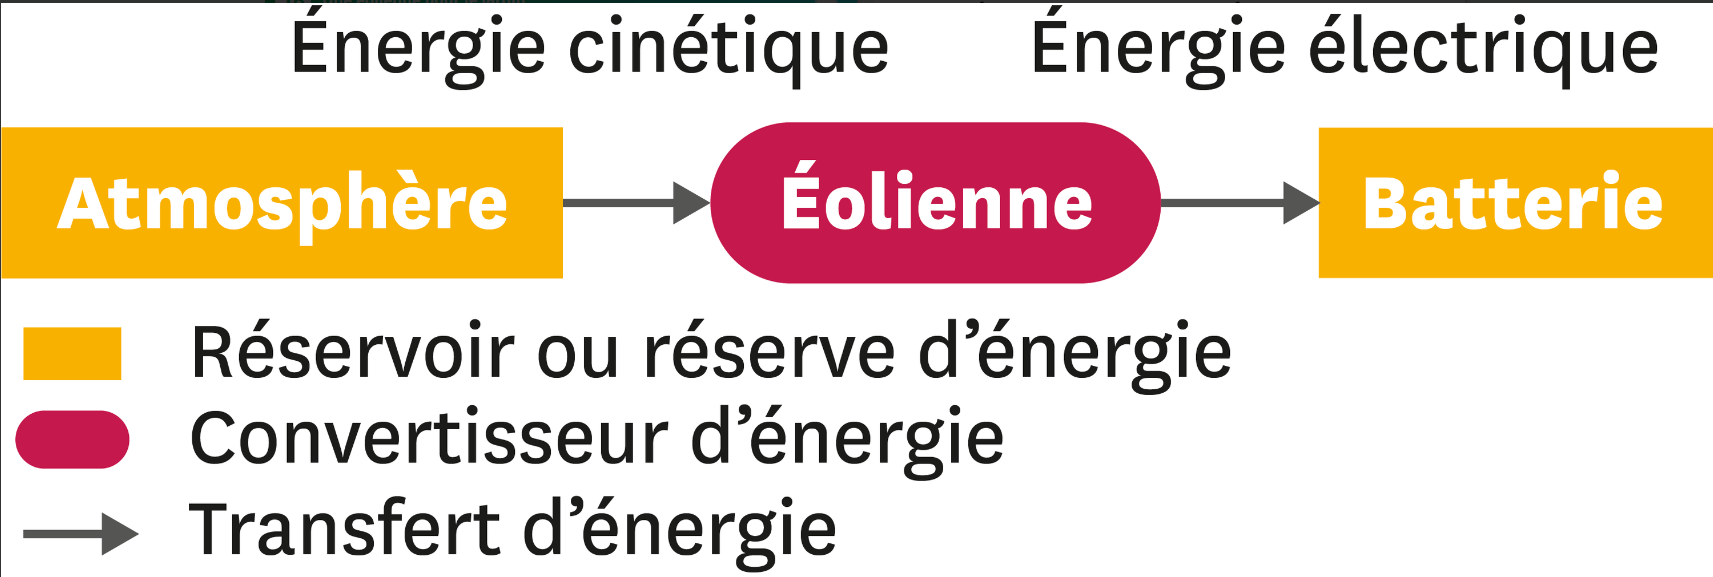
\includegraphics[scale=0.2]{img/chaine}
			\end{center}
		\end{solution}
	
\end{questions}